\documentclass[11pt,titlepage,fleqn]{article}
\usepackage[T1]{fontenc}
\usepackage{xcolor}
\usepackage{mdwlist}
\usepackage[pagestyles]{titlesec}
\usepackage{fancyhdr}
\usepackage{amsmath}
\usepackage[top=1in, bottom=1in, left=1in, right=1in] {geometry}
\usepackage{graphicx} 
\usepackage{enumerate}
\usepackage{setspace}
\usepackage{hyperref}
\graphicspath{{./figures/}}

\renewcommand{\baselinestretch}{1.5}

\textwidth 444pt
\textheight 660pt
\oddsidemargin 15pt
\evensidemargin 15pt

\newcommand{\rmd}{\mathrm{d}}

\usepackage{listings}
\lstset{% setup parameters for listings:
  columns=fullflexible,  % avoids addition of extra spaces in unexpected positions
  keepspaces,            % causes alignment-by-spaces to be preserved in output
  basicstyle=\ttfamily,  % With fullflexible and keepspaces, using a non-monospaced
                         % font causes incorrect alignment of plain-text columns.
  backgroundcolor=\color{gray!10},
  keywordstyle=\bfseries\color{black!90},
  numbers=none, numberstyle=\small\sffamily, numbersep=5pt,
  extendedchars=true}
\lstset{language=Bash}


\begin{document}

\pagestyle{fancy} \lhead{{\bf \Large}}
\lhead{\bf GEO441 - Computational Geophysics} 
\rhead{\bf April 16, 2025} \renewcommand{%
\headrulewidth}{0.5 pt}


\begin{center}
{\Large {\bf Problem Set 9}}
\end{center} 

\begin{tabular}{@{}p{1.8in}p{4in}}
\bf{Submission deadline:} & April 23, 2025 \\            
\bf{Submission type:} & Report (soft or hard copy) and source code (soft copy)  
\end{tabular}

\section*{Spectral Element Method}

Solve the 2D wave equation using \texttt{SPECFEMPP}. Compare the seismograms and wavefield snapshots for simulations with different number of elements and/or GLL points.

\section*{Model description}

\begin{figure}[htbp]
\centering
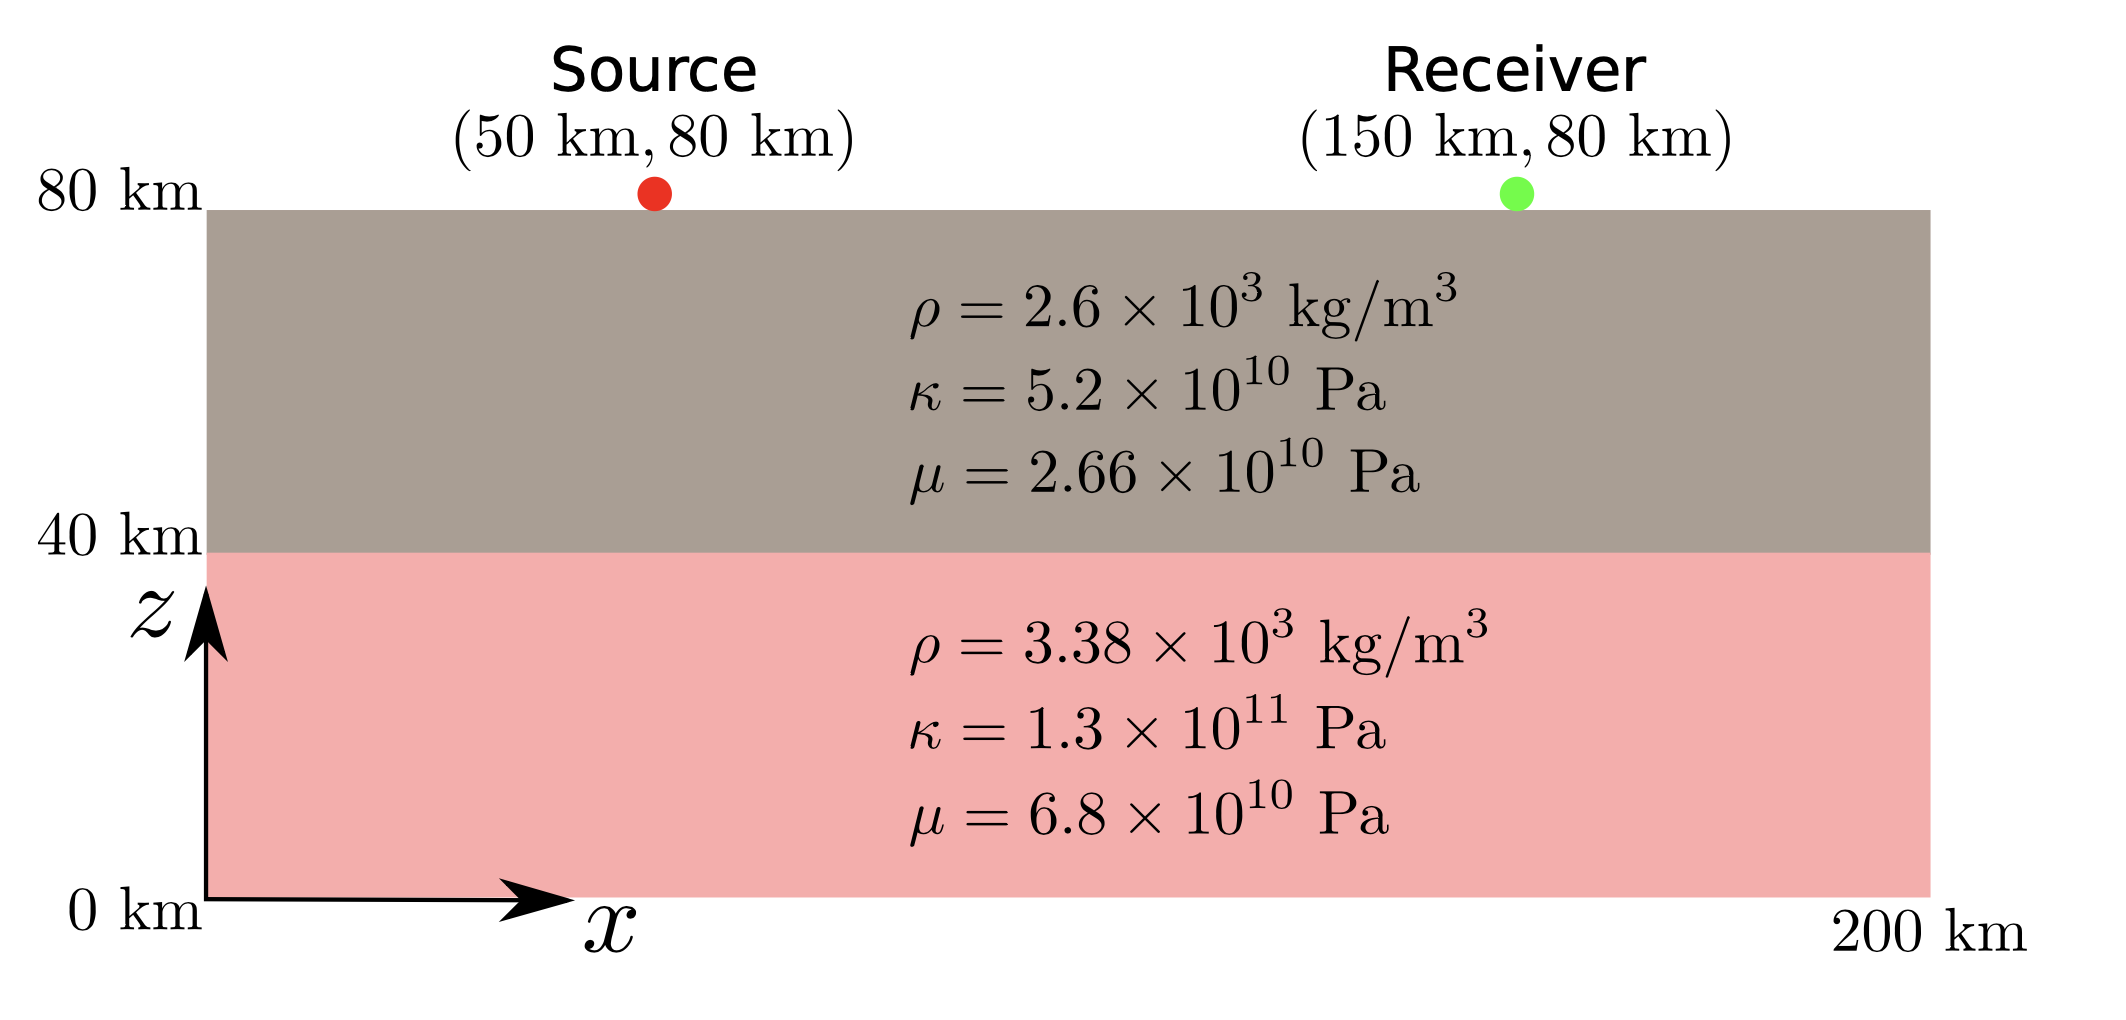
\includegraphics[width=\textwidth]{model.png}
\caption{2D model for the wave propagation.}
\label{fig:model}
\end{figure}

The model consists of two layers as shown in Figure~\ref{fig:model}. The elastic properties of each layer are inscribed on the corresponding layer. Similarly, the source and the receiver locations are shown in the model with a red and a green circles, respectively.
    
\section*{Instructions}

We will be using the software \texttt{SPECFEMPP} to simulate wave propagation with the spectral-element-method. \texttt{SPECFEMPP} is \texttt{C++} software relying on \texttt{Kokkos} to implement performance-portable code. To compile the software we need a couple of packages that are standard on most systems:
\begin{itemize}
	\item \texttt{cmake}
	\item \texttt{C} compiler
	\item \texttt{Fortran} compiler
	\item \texttt{C++} compiler
	\item Optional: \texttt{VTK} -- the visualization toolkit for plotting snapshots.
\end{itemize}

Since you will be working with Adroit, you do not have to worry about these dependencies because they are already installed. In fact, this utilities are usually installed by default in most LINUX systems. Under WINDOWS, one may use LINUX Subsytem (WSL) or Cygwin (www.cygwin.com), or MinGW (www.mingw.org) to install the software.

\begin{enumerate}

\item Optional: Login to Adroit\\
{\bf ssh <NetId>@adroit.princeton.edu}       
    
\item Clone the repository\\
      {\bf git clone https://github.com/PrincetonUniversity/SPECFEMPP.git \newline \text{-}\text{-}branch devel \text{-}\text{-}single-branch}
\item Enter directory\\
      {\bf cd SPECFEMPP}       
		
\item Export the VTK build directory location for compilation\\
      {\bf export VTK\_DIR=/scratch/network/lsawade/vtk/build}

\item Load appropriate compiler\\
      {\bf module load gcc-toolset/10}

\item Configure the \texttt{SPECFEMPP}\\
      {\bf cmake \text{-}\text{-}preset release}

\item Compile the \texttt{SPECFEMPP}\\
      {\bf cmake \text{-}\text{-}build \text{-}\text{-}preset release \text{-}j}

\item Add the compiled binary folder to PATH variable so that you can use commands \\{\bf xmeshfem2D} and {\bf specfem2d} directly.\\
      {\bf export PATH=\$PATH:\$PWD/build/release/bin}

\item Now before we can run the software we need some parameter files, which are distributed as part of the class, but also are located at {\bf /home/GEO441/hw9\_data.tar} on Adroit. So either \\
      {\bf tar -xvf /home/GEO441/hw9\_data.tar}\\
    Or, copy it from the modules on Canvas and copy it to Adroit.
      
\item Enter the directory
      {\bf cd GEO441}

\item Create output folders\\
      {\bf mkdir -p OUTPUT\_FILES/results}\\
      {\bf mkdir -p OUTPUT\_FILES/display}\\
      {\bf mkdir -p OUTPUT\_FILES/wavefield}
      
\item Run the software
  \begin{itemize}
    \item Run the mesher:\\
          {\bf xmeshfem2D -p Par\_file}
    \item Run the solver:\\
          {\bf specfem2d -p specfem\_config.yaml}
  \end{itemize}

\item  Plotting results

\noindent Further parameters are documented here:\\
\phantom{ } \url{https://specfem2d-kokkos.readthedocs.io/en/devel/}

  \begin{enumerate}
    \item Seismograms (ASCII format) are stored in the folder {\bf OUTPUT\_FILES/results}. File names for the seismograms have the form: \\
        {\bf  <Network>.<Station>.S2.BX<Component>.semd}. \\
        The files have timestamp in the first and value in the second column, and can be read and plotted using Python or Matlab for example.

    \item Wavefield images and full wavefield data (ASCII format) are off by default by if activate stored in the folder {\bf OUTPUT\_FILES/display}. If the {\bf specfem\_config.yaml} is updated as follows


\newpage
\begin{lstlisting}
...
writer:
  seismogram:
    format: ascii
    directory: OUTPUT_FILES/results

  wavefield:
    directory: "OUTPUT_FILES/wavefield"
    format: ASCII
    time_interval: 1000

  display:
    format: PNG
    directory: OUTPUT_FILES/display
    field: displacement
    simulation-field: forward
    time-interval: 100
...
\end{lstlisting}
         The image files have the format {\bf wavefield<timestamp>.png} and can be viewed using \url{myadroit.princeton.edu} and/or copied to your local machine using {\bf scp} or using VSCode remote development.
   
  \end{enumerate}

\end{enumerate}


\section*{Assignment}

\begin{enumerate}

\item Plot the seismograms and snapshots for both SH and PSV, respectively.

\item Modify number of elements ({\bf NEX}, {\bf NEZ}) to see how the seismograms change for both SH and
PSV forces. The "{\bf number of grids per wavelength}" on the screen output is an indication of the accuracy of the simulation.
\item (bonus) Plot the wavefield using your own tools from {\bf OUTPUT\_FILES/wavefield}.
        
\end{enumerate}

You are encouraged to play around setting different source and receiver locations, etc.

\end{document}
